% =============================================================================
% Results -- RQ1 (final decisions).  Drafted 2026-07-26.
%
% Figure file: plots/rq1_outcomes/Decision_final.pdf  (a .png of the same name
% sits beside it; use the PDF -- it is vector and embeds TrueType, not Type 3).
%
% TYPE SIZE.  This is a ONE-COLUMN figure.  Decision_final.pdf is authored at
% 3.30 x 5.35 in -- 3.30 in IS \columnwidth -- so width=\columnwidth is a 1.0x
% no-op and authored pt = printed pt: 9.5pt model names / ticks / numerals /
% legend / band headers, 10.5pt panel titles.  All clear AAAI's 9pt in-figure
% minimum with half a point of margin.
%
% DO NOT promote this to figure* / width=\textwidth without regenerating.
% Scaling a 3.3in figure up to 7.0in would blow the type to ~20pt; scaling a
% 7.0in figure down to \columnwidth (which is what happened on 2026-07-28)
% shrinks 9-10pt source text to 4-5pt and BREAKS the 9pt rule.  Author at the
% width the figure is actually placed at.  If the layout changes, edit
% FIG_W in analysis/plot_rq1_outcomes.py and re-run it.
%
% No in-figure title -- the \caption below is the title (SHOW_TITLE=False).
%
% Numbers regenerable via analysis/plot_rq1_outcomes.py. Accuracies are
% end-to-end (a response that never commits is scored as a failure) unless
% stated otherwise.
% =============================================================================

\section{Results}

\subsection{RQ1: Are Final Decisions Optimal?}

We first ask whether the model commits to the action the baseline prescribes.
The measurement is the parsed final answer emitted after the model has written
its own chain of thought: a single binary commitment, scored against the
Bayesian-optimal action for that history. Unlike the logit-level probes, this
outcome is deterministic --- the model either selects the optimal action or it
does not.

\begin{figure}[t]
    \centering
    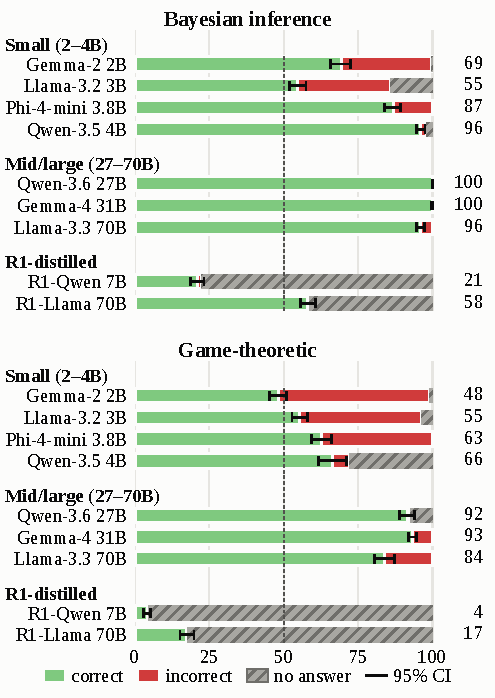
\includegraphics[width=\columnwidth]{plots/rq1_outcomes/Decision_final.pdf}
    \caption{Final decisions made by nine models in Bayesian and game-theoretic
    scenarios, showing correct, incorrect and no-response rates. Shares are
    balanced over the two baseline-optimal action classes, so chance is $50\%$;
    error bars are $95\%$ bootstrap confidence intervals resampling sessions.}
    \label{fig:decision-final}
\end{figure}

Figure~\ref{fig:decision-final} decomposes every unambiguous decision step into
three outcomes: \emph{correct}, \emph{incorrect}, and \emph{no answer} --- a
response that exhausts the generation budget without committing to a decision.
All three are reported because the failures are not interchangeable, and because
accuracy computed only over responses that terminate silently re-weights the
denominator toward the steps a model finds easy.

\textbf{\textit{Decision quality improves with scale, but the floor it improves
from depends on the scenario family.}}
Qwen-3.6 27B and Gemma-4 31B are close to the baseline throughout: $100$ and
$99.9$ on the Bayesian-inference scenarios and $91.6$ and $93.4$ on the
game-theoretic ones, with no individual scenario below $85$. The smallest models
are not. Llama-3.2 3B is barely separable from chance in either family ($54.7$
$[51.9,57.5]$ and $55.4$ $[52.8,57.9]$), and Gemma-2 2B is \emph{indistinguishable}
from chance on the game-theoretic scenarios, its interval $48.1$ $[45.3,50.8]$
containing $50$. Phi-4-mini 3.8B is the exception within that band, reaching
$86.8$ on Bayesian inference: small scale alone does not preclude competent
inference-driven decisions.

\textbf{\textit{Model family matters as much as parameter count.}}
Qwen-3.5 4B attains $96.1$ $[94.7,97.5]$ on the Bayesian-inference scenarios,
identical to Llama-3.3 70B ($96.1$ $[94.7,97.4]$) at roughly one-twentieth the
size. In the other direction, Llama-3.3 70B is the largest non-distilled model we
evaluate and still trails both mid-sized models on the game-theoretic scenarios
($83.9$ against $91.6$ and $93.4$). Scale alone does not order these models.

\textbf{\textit{The reasoning-distilled models fail by never committing.}}
R1-Qwen 7B and R1-Llama 70B are almost never wrong --- incorrect decisions
account for $1.5\%$ and $0.6\%$ of Bayesian steps and $0.4\%$ and $0.3\%$ of
game-theoretic steps, the lowest error rates in the suite --- and almost never
decided. Their no-answer shares are $77.7\%$ and $41.3\%$ on Bayesian inference
and $95.5\%$ and $82.3\%$ on the game-theoretic scenarios, leaving end-to-end
accuracies of $20.9$ and $58.1$, and $4.1$ and $17.4$. Every such response
exhausts the $2048$-token budget, and most carry explicit backtracking
(``wait'', ``let me reconsider'') as the model relitigates a conclusion it has
already reached rather than stating it. The rate is flat across decision steps
($88$--$98\%$ at every step for R1-Qwen 7B), so it does not track how much
history there is to process: this is non-convergence rather than a budget that
happens to be too small. Scaling the distillation from 7B to 70B restores
commitment on the inference scenarios but not on the game-theoretic ones.

\textbf{\textit{Non-termination is not confined to the distilled models.}}
Qwen-3.5 4B fails to commit on $27.9\%$ of game-theoretic steps, which is what
separates its $91.8$ accuracy over terminated responses from $66.3$
$[61.8,71.1]$ end-to-end. Its non-termination behaves differently, however:
it rises with the length of the history ($6\%$ at the second decision step to
$40\%$ at the tenth) and its truncated responses are coherent rather than
repetitive, so it reflects the generation budget interacting with a verbose
derivation rather than an inability to conclude.

Every model is less accurate under game-theoretic structure than under Bayesian
inference, and the gap does not close with scale. RQ2 and RQ3 ask where in the
decision process it originates.
